% This file was created with tikzplotlib v0.10.1.
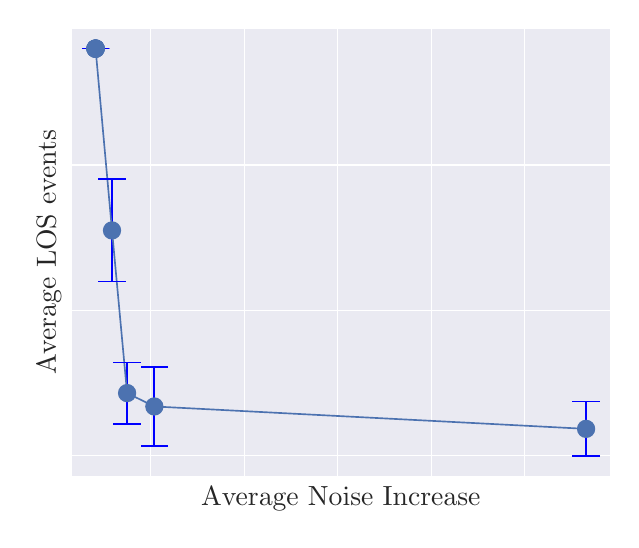
\begin{tikzpicture}

\definecolor{darkslategray38}{RGB}{38,38,38}
\definecolor{lavender234234242}{RGB}{234,234,242}
\definecolor{steelblue76114176}{RGB}{76,114,176}

\begin{axis}[
axis background/.style={fill=lavender234234242},
axis line style={white},
tick align=outside,
x grid style={white},
xlabel=\textcolor{darkslategray38}{Average Noise Increase},
xmajorgrids,
xmajorticks=false,
xmin=20.5736539429203, xmax=23.4601925168384,
xtick style={color=darkslategray38},
y grid style={white},
ylabel=\textcolor{darkslategray38}{Average LOS events},
ymajorgrids,
ymajorticks=false,
ymin=-1.41708654632227, ymax=29.400813645063,
ytick style={color=darkslategray38}
]
\path [draw=blue, thick]
(axis cs:23.3289862180239,-0.0162729012593024)
--(axis cs:23.3289862180239,3.7362729012593);

\path [draw=blue, thick]
(axis cs:21.0196410444504,0.679705898252911)
--(axis cs:21.0196410444504,6.12029410174709);

\path [draw=blue, thick]
(axis cs:20.8738832353825,2.20869708473654)
--(axis cs:20.8738832353825,6.43130291526346);

\path [draw=blue, thick]
(axis cs:20.7931684962753,11.9857433218389)
--(axis cs:20.7931684962753,19.0142566781611);

\path [draw=blue, thick]
(axis cs:20.7052091136627,28)
--(axis cs:20.7052091136627,28);

\path [draw=blue, thick]
(axis cs:20.7052740554892,28)
--(axis cs:20.7052740554892,28);

\path [draw=blue, thick]
(axis cs:20.7051515069496,28)
--(axis cs:20.7051515069496,28);

\path [draw=blue, thick]
(axis cs:20.7049231104863,28)
--(axis cs:20.7049231104863,28);

\path [draw=blue, thick]
(axis cs:20.7052832510215,28)
--(axis cs:20.7052832510215,28);

\path [draw=blue, thick]
(axis cs:20.7048938152846,28)
--(axis cs:20.7048938152846,28);

\path [draw=blue, thick]
(axis cs:20.7048602417347,28)
--(axis cs:20.7048602417347,28);

\addplot [semithick, blue, mark=-, mark size=5, mark options={solid}, only marks]
table {%
23.3289862180239 -0.0162729012593024
21.0196410444504 0.679705898252911
20.8738832353825 2.20869708473654
20.7931684962753 11.9857433218389
20.7052091136627 28
20.7052740554892 28
20.7051515069496 28
20.7049231104863 28
20.7052832510215 28
20.7048938152846 28
20.7048602417347 28
};
\addplot [semithick, blue, mark=-, mark size=5, mark options={solid}, only marks]
table {%
23.3289862180239 3.7362729012593
21.0196410444504 6.12029410174709
20.8738832353825 6.43130291526346
20.7931684962753 19.0142566781611
20.7052091136627 28
20.7052740554892 28
20.7051515069496 28
20.7049231104863 28
20.7052832510215 28
20.7048938152846 28
20.7048602417347 28
};
\addplot [semithick, steelblue76114176, mark=*, mark size=3, mark options={solid}]
table {%
23.3289862180239 1.86
21.0196410444504 3.4
20.8738832353825 4.32
20.7931684962753 15.5
20.7052091136627 28
20.7052740554892 28
20.7051515069496 28
20.7049231104863 28
20.7052832510215 28
20.7048938152846 28
20.7048602417347 28
};
\end{axis}

\end{tikzpicture}
